%%%%%%%%%%%%%%%%%%%%%%
\section{Implementation}
%%%%%%%%%%%%%%%%%%%%%%

To create a scalable FPGA implementation, the design used the following general guidelines:

\begin{enumerate}
    \item Block RAMs for queue storage to simplify logic and routing
    \item Clock cycle-efficient search, insert, and remove operations 
    \item Scalable and parallelizable processing to achieve a performance target given a clock frequency
\end{enumerate}

Given the above guidelines, we opted for the following design elements to build our PIFO:
\begin{enumerate}
    \item A deterministic skip list as the queue data structure
    \item A small high-speed cache implemented in registers
    \item A scalable number of parallel priority queues, each consisting of both (1) and (2)
    \item Additional design features including four pointers per skip list node, independent pointer memories, and enqueue throttling for low dequeue latency
\end{enumerate}

\subsection{Top Level PIFO}\label{sec:pifo}

The PIFO is the top level element that is responsible for scheduling the packet descriptors at line rate. As shown in Figure \ref{fig:pifo-top}, the PIFO is composed of one or more parallel priority queues. The implementation details of our priority queue is described in section~\ref{sec:priority-queue}. At a high level, each priority queue is essentially a PIFO that can perform dequeues at line rate and enqueues at less than line rate. We construct a single line rate PIFO by combining these priority queues in parallel and load balancing across them.

During an enqueue operation, the PIFO will examine each priority queue that is available and enqueue into the one with the least number of packet descriptors. This allows the enqueue load to be balanced across all priority queues and avoids overwhelming any one queue. As long as each priority queue has a bounded enqueue latency, we can be sure to use enough parallel queues to guarantee line rate performance of our PIFO. As explained in section \ref{sec:skip-list-impl}, this is indeed the case.

During a dequeue operation, the PIFO examines the head element of each priority queue and removes the one with the smallest rank. The PIFO breaks ties using the enqueue timestamp appended to the packet descriptor in order to guarantee FIFO ordering of packets with the same rank.

\begin{figure}[!ht]
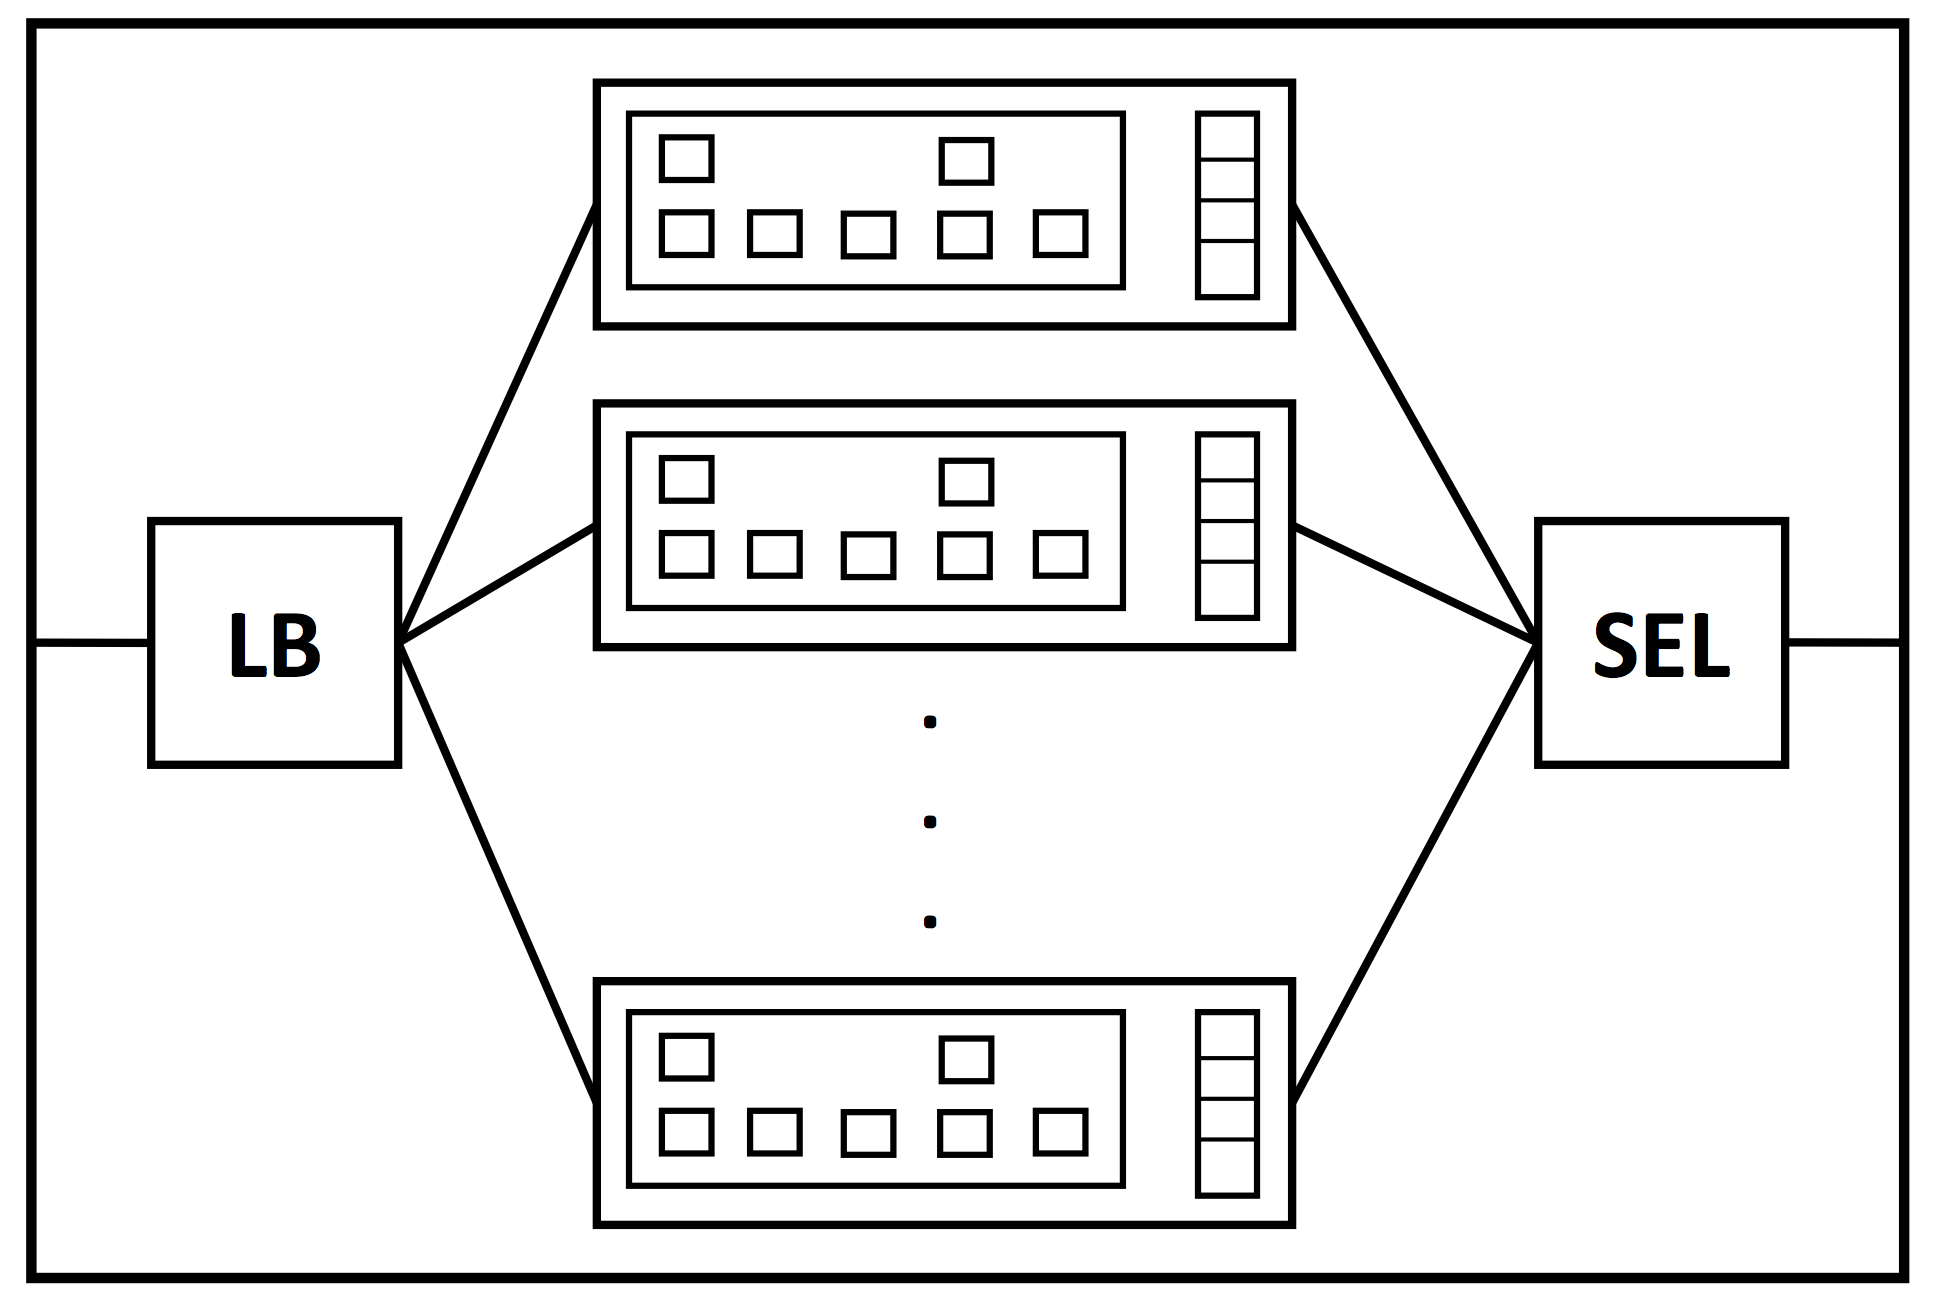
\includegraphics[width=0.8\linewidth]{figures/design/pifo-top}
\caption{Top level PIFO block diagram. LB is the enqueue load balancing module and SEL is the dequeue selector module.}
\label{fig:pifo-top}
\end{figure}

\begin{figure}[!ht]
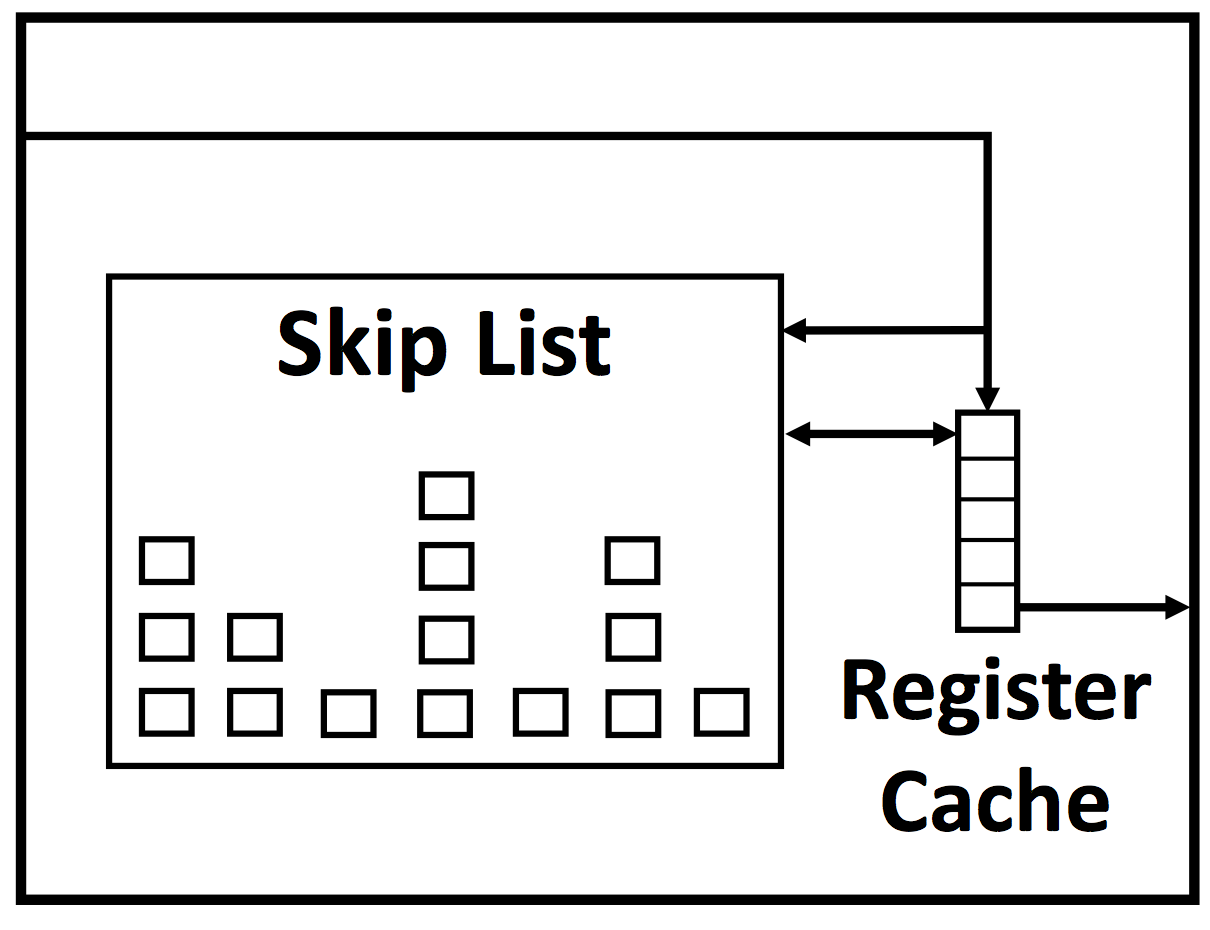
\includegraphics[width=0.7\linewidth]{figures/design/priority-queue}
\caption{Priority queue block diagram}
\label{fig:priority-queue}
\end{figure}

\subsection{Priority Queue}\label{sec:priority-queue}

The priority queue that we have designed is in fact a PIFO that can be drained at line rate and filled at sub-line rate. It sorts packet descriptors in the order of decreasing rank values. Figure \ref{fig:priority-queue} shows the top level priority queue which is composed of a register-based cache and a skip list. Each of these components is explained in more detail in sections \ref{sec:reg-cache} and \ref{sec:skip-list-impl}, respectively. Once again, the register cache and the skip list are both PIFOs, each with different enqueue and dequeue properties. The size of the cache is on the order of $log_2$ the size of the skip list and can support one enqueue and one dequeue every other cycle. The latency for an enqueue operation into the skip list is also logarithmic in the number of packet descriptors that are currently in the skip list. It typically takes one or two orders of magnitude longer than an enqueue into the cache for a skip list with a fill level of approximately 2000 packet descriptors. A dequeue from the skip list is also affected by its current size, but it is typically much faster than an enqueue. Furthermore, in order to maintain a simple skip list implementation, the design serializes enqueue and dequeue operations for the skip list.

%\todo[inline]{Explain requirements for line rate performance. Don't let output register drain. How do we guarantee this?}

% Algorithm~\ref{alg:enq-proc} describes the procedure for inserting an element into the priority queue...

%Algorithm~\ref{alg:busy-proc} describes the procedure for generating the priority queue's busy signal, which prevents the top level PIFO from attempting to enqueue anything into the priority queue...

%It could be the case that a single priority queue receives all of the smallest ranks... requires a single priority queue to drain at line rate.


%\begin{algorithm}
%\footnotesize
%\caption{Priority Queue Busy Signal Generation}\label{alg:busy-proc}
%\begin{algorithmic}[1]
%  \If{$skip\_list.busy$}
%    \State $busy = 1$
%  \Else
%    \State // $skip\_list.enq\_delay$ measured in increments of 12.8 cycles
%    \If{$skip\_list.enq\_delay > out\_reg.size$}
%      \State $busy = 1$
%    \Else
%      \State $busy = 0$
%    \EndIf
%  \EndIf
%\end{algorithmic}
%\end{algorithm}


\subsection{Fast Register-based Cache}\label{sec:reg-cache}

We use a small cache implemented using registers to significantly reduce the average enqueue and dequeue times.  The packet ranks stored in the cache are not ordered and the cache continuously advertises the minimum and maximum ranks stored in it. If the cache is full, when a new value is enqueued, it is compared with the maximum rank in the cache and then inserted in the skip list (when the new value is larger) or in the cache replacing the maximum value, which is sent to the skip list (when the new value is smaller). The cache insertion logic is shown in Algorithm \ref{alg:enq-proc}.

\begin{algorithm}
\footnotesize
\caption{Cache Insertion Procedure}\label{alg:enq-proc}
\begin{algorithmic}[1]
  \State \underline{For every arriving packet: $p$}
  \If{$cache.size < cache.max\_size \And skip\_list.size = 0$}
   \State $cache.insert(p)$
  \Else 
    \If{$p.rank < cache.max\_rank$}
     \State $skip\_list.insert(cache.max\_rank)$
     \State $cache.insert(p)$
    \Else
     \State $skip\_list.insert(p)$
    \EndIf
  \EndIf
\end{algorithmic}
\end{algorithm}

The cache is sized to hold at least $log_2$ the number of elements that can be stored in the skip list.  This size accommodates the fill level required for the starvation prevention mechanism mentioned in section \ref{sec:add-features}.

\subsection{Skip List}\label{sec:skip-list-impl}

The key to implementing a scalable PIFO is to find an appropriate data structure that facilitates simple insertion operations and fast in-order removal operations.

The skip list was first described in 1990~\cite{skip-list-1990} as a probabilistic alternative to balanced trees. They are attractive because of their simple implementation and fast insert and remove operations, which, on average, take logarithmic running time in $n$, the number of elements. The probabilistic nature of skip lists, however, means that the worst-case performance is unbounded. This is unacceptable because we require guaranteed line rate performance with our PIFO. 

Deterministic skip lists~\cite{det-skip-list} retain the simple implementation details of their probabilistic counterparts, while bounding the insertion and removal operations to functions of $\log n$. They are able to achieve this by enforcing a few simple rules upon insertion and removal to ensure that the skip list maintains a regular structure that bounds the worst-case insertion and removal times. Figure \ref{fig:skip-list-a} shows an example 1-2-3 skip list and the path that would be taken to insert element 29 into the data structure. The insertion operation always starts at the top level's tail element. It then skips across the top level until seeing that the next element is less than or equal to the value being inserted at which point it drops down a level. This process continues until reaching the insertion position in the bottom level. The 1-2-3 skip list structure policy enforces that there are no more than three consecutive nodes at the same level. Therefore, since our insertion operation caused the skip list to violate this structure requirement, we must add a level to node 18 in the third level and to node 26 in the second level. The resulting skip list is shown in Figure \ref{fig:skip-list-b}.
\paragraph{Worst-case insertion time} 
In a 1-2-3 skip list with $L$ levels, the worst-case insertion time occurs when three consecutive nodes are encountered at each level, requiring the addition of a node at each level.  
The operations that are performed are: 
\begin{itemize}
\item At each level:
\begin{itemize}
\item 3 node reads
\item 1 balancing node insertion
\end{itemize}
\item 1 new node insertion
\end{itemize}
Each node insertion requires two write operations, one for the node being added and one for the neighboring node or nodes\footnote{Multiple nodes can be written simultaneously as described in section \ref{sec:add-features} }.
The worst-case insertion time is given by
\begin{equation}\label{worst-case-insert_eqn}
(3 T_{Rd} + 2 T_{Wr} + K_{1}) (L - 1) + 2 T_{Wr} + K_{2}
\end{equation}
where:\\
\indent $T_{Rd}$ = node read time\\
\indent $T_{Wr}$ = node write time\\
\indent $K_{1}$, $K_{2}$ = processing overhead\\

\begin{figure*}[t!] % "[t!]" placement specifier just for this example
\centering
\begin{subfigure}{\linewidth}
\centering
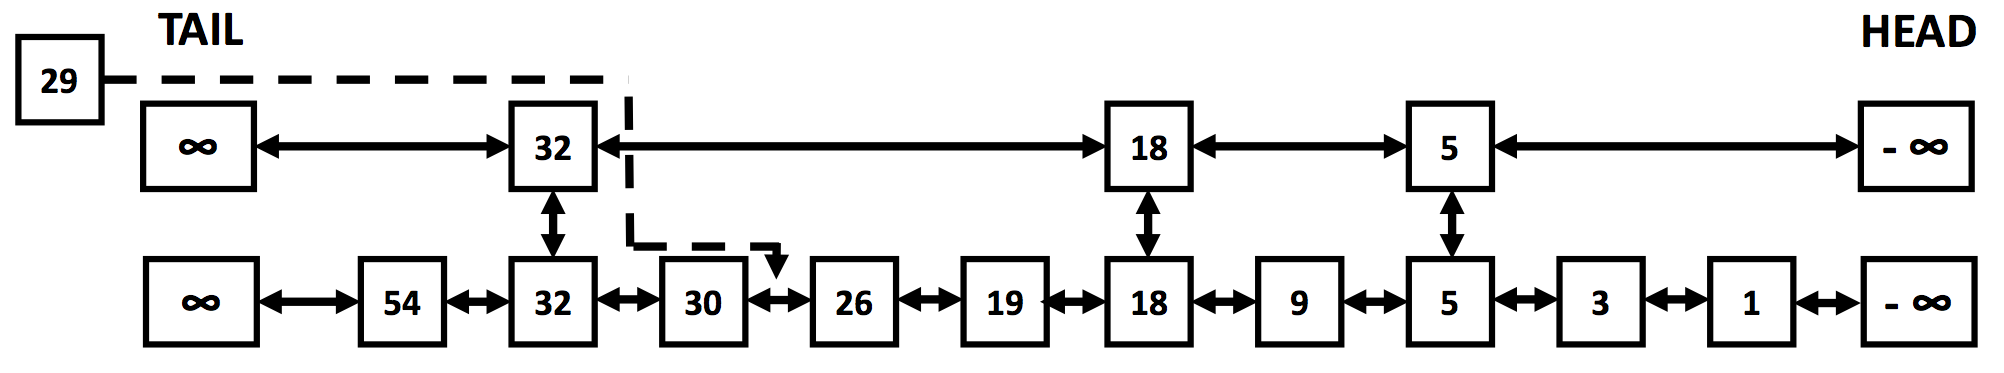
\includegraphics[width=0.8\linewidth]{figures/design/skip-list-a}
\caption{Original 1-2-3 skip list and the path to insert element 29.} \label{fig:skip-list-a}
\end{subfigure}\hspace*{\fill}

\medskip
\begin{subfigure}{\linewidth}
\centering
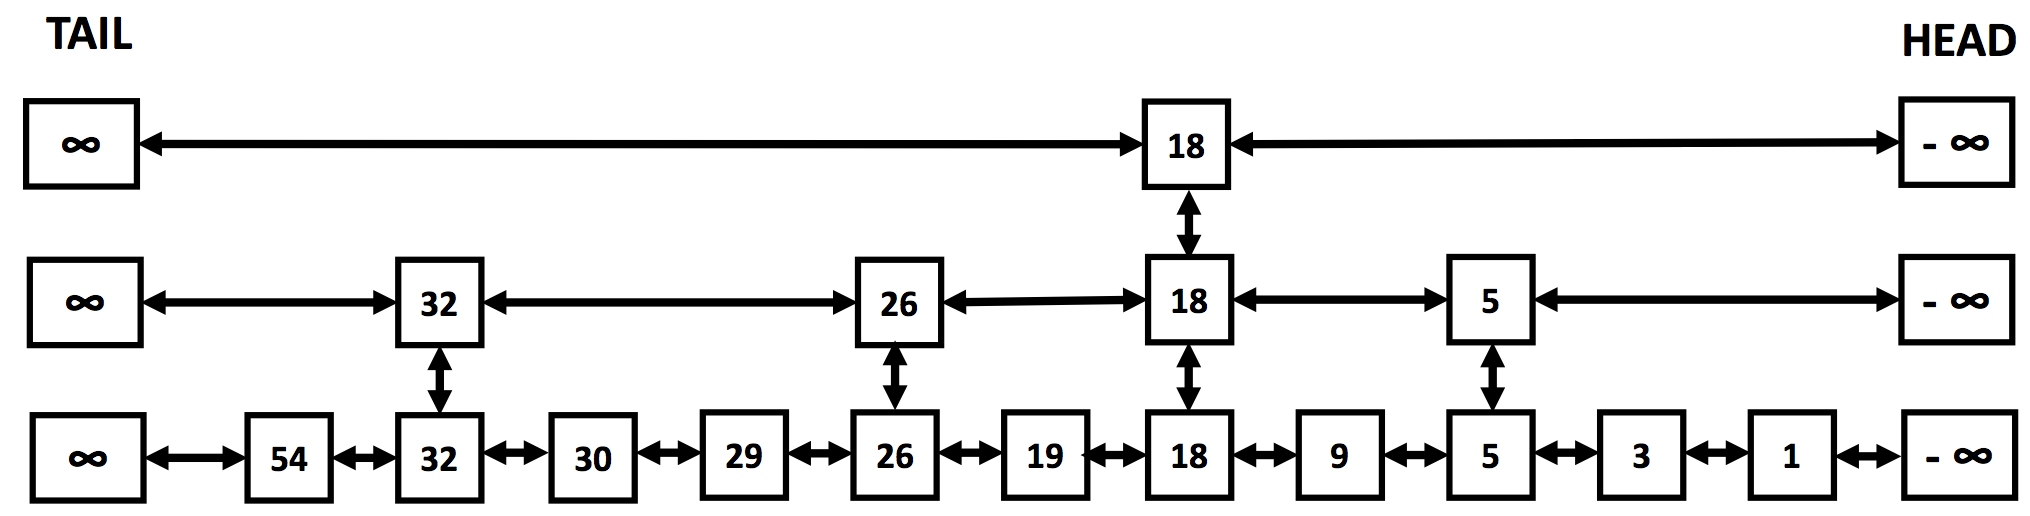
\includegraphics[width=0.8\linewidth]{figures/design/skip-list-b}
\caption{Final 1-2-3 skip list after inserting element 29.} \label{fig:skip-list-b}
\end{subfigure}\hspace*{\fill}

\caption{Insertion into a 1-2-3 deterministic skip list.}\label{fig:skip-list}
\vspace{-1.0em}
\end{figure*}

The astute reader will recall that elements are always dequeued from the head of a PIFO. This means that if we use a skip list as the underlying primitive with which to implement a PIFO then the removal operation becomes trivial, simply remove the head element.  There is no complicated re-balancing logic that must take place.

\subsubsection{Additional Design Features}\label{sec:add-features}
The following design features were used to improve performance
\paragraph{Skip List Pointers}
A standard skip list uses two pointers:
\begin{itemize}
\item A $right$ pointer to move forward from the tail towards the head
\item A $down$ pointer to move from any level to the base level
\end{itemize}
We added two pointers, $left$ and $up$ to speed up the dequeue operation, including freeing nodes from upper levels if any.

Since every enqueue operation starts by reading the tail node at the top level and every dequeue by reading the head node at the bottom level, we store these pointers in registers to eliminate a block RAM access.

In addition, we used separate memories for each of the four pointers, which allows us to update different pointers for different nodes in a single clock cycle.  For example, when adding a new node for balancing, pointers on the left, right, and down neighboring nodes are updated in a single clock cycle.

\paragraph{Enqueue Throttling}\label{enq-throttle}
As locations in the cache become vacant due to dequeues, they are replenished from the head of the skip list as a background process.  If a cache insertion and a removal coincide, the insertion takes precedence and the replenishment of the cache is delayed.  To prevent cache starvation under high enqueue rates, we introduced an enqueue throttling mechanism that maintains a cache fill level such that the cache will not become empty if the replenishment is blocked for a worst-case enqueue time.  

The throttling is activated using a dynamic threshold that is a function of the fill level of the skip list.  The net effect is that the fill level of the cache varies with the fill level of the skip list; if the skip list is more full, enqueue time is longer and therefore we need more descriptors in the cache to maintain the dequeue rate.  The enqueue throttling allows sustained dequeuing from a single priority queue every four clock cycles while not adversely affecting the enqueue latency. We have used the following thresholds for controlling the cache fill level as a function of the skip list fill level (up to 2048 descriptors).

\begin{center}
\begin{tabular}{|c|c|}
    \hline
    \textbf{Skip List Fill Level} & \textbf{Cache Fill Level} \\
    \hline
    0 & 0\\
    \hline
    1 & 1\\
    \hline
    2 - 3 & 2\\
    \hline
    4 - 7 & 3\\
    \hline
    8 - 15 & 4\\
    \hline
    16 - 31 & 5\\
    \hline
    32 - 63 & 6\\
    \hline
    64 - 127 & 7\\
    \hline
    128 - 255 & 8\\
    \hline
    256 - 511 & 9\\
    \hline
    512 - 1023 & 10\\
    \hline
    1024 - 2047 & 11\\
    \hline
\end{tabular}
\end{center}

It is not surprising that the cache fill level is a logarithmic function of the skip list fill level, since the skip list enqueue time is also a logarithmic function of the fill level.

\subsection{Multi-Port Scheduler Design}\label{sec:sched-des}

This section describes how to build a multi-port scheduler utilizing the line rate PIFO design described in the previous sections. We propose to use a virtual output PIFO queuing architecture. This means that each PIFO must support both insertions and removals at line rate in order to sustain the worst case traffic patterns. 

%\subsubsection{NetFPGA Platform}

%The NetFPGA SUME is a {4x10Gb/s} networking hardware platform that provides programmability via a Virtex-7 FPGA. The NetFPGA reference design runs at a core clock frequency of 200 MHz using a 256-bit datapath; fast enough to support more than 40Gb/s. Figure XXX shows a block diagram of how we integrated our scheduler into the NetFPGA reference design. The reference design that we used consists of four input ports and four output ports, each running at 10Gb/s. An input arbiter performing deficit round robin scheduling reads packets out of the input queues and injects them into the core datapath. The output port lookup module is responsible for deciding the packet's destination port, rank, and queue ID. These three decisions are passed along with the packet to our scheduling block, which then makes the appropriate scheduling decision and forwards packets to appropriate the output port.

%\todo[inline]{insert NetFPGA reference design with scheduler.}

\subsubsection{Top Level Scheduler Design}\label{sec:top-level-sched}

Figure \ref{fig:tm-top} shows a block diagram of our top level scheduler design. The design uses a virtual output PIFO queuing architecture, such that there is one PIFO for each output port at each of the input ports. Each input port also has a partition of packet buffer storage which is shared amongst all of the PIFOs at that port. Full packets are stored in the packet buffer and packet descriptors are enqueued into and scheduled by the PIFOs. Assuming that packets are not broadcast or multicast, the packet buffer as well as each PIFO must be fast enough to perform both enqueue operations and dequeue operations at exactly line rate, or 10Gb/s for our design. The line rate and clock frequency directly dictate the maximum number of clock cycles alloted to process each packet in order to guarantee line rate performance. Our design uses a 200 MHz clock, which means that the maximum number of clock cycles to process each packet is determined by the following equation,

$$ \frac{(8~B + 64~B + 12~B)\times 200~MHz}{10~Gb/s} = 13.44~\mbox{cycles} $$

This assumes the minimum size packet is 64B and there is an 8B preamble and Start of Frame Delimiter and a 12B interframe gap. The above result enforces a hard constraint on the design of our PIFO which must be able to both enqueue and dequeue a packet descriptor once every 13.44 cycles. Additionally, the packet buffer must be able to enqueue and dequeue 64B packets every 13.44 cycles. 

In addition to the PIFO and packet buffer, the design also consists of a PIFO selector module at each output port. This module is responsible for comparing the rank values at the head of its corresponding virtual output PIFOs to decide which packet to transfer into the output queue. The selector will dequeue the packet with the smallest rank. Each packet descriptor is also accompanied by an enqueue timestamp, which is used to break ties in cases where there are identical ranks across virtual output PIFOs. This timestamp allows the scheduler to guarantee that packets configured with the same rank depart in FIFO order.


\begin{figure}[!h]
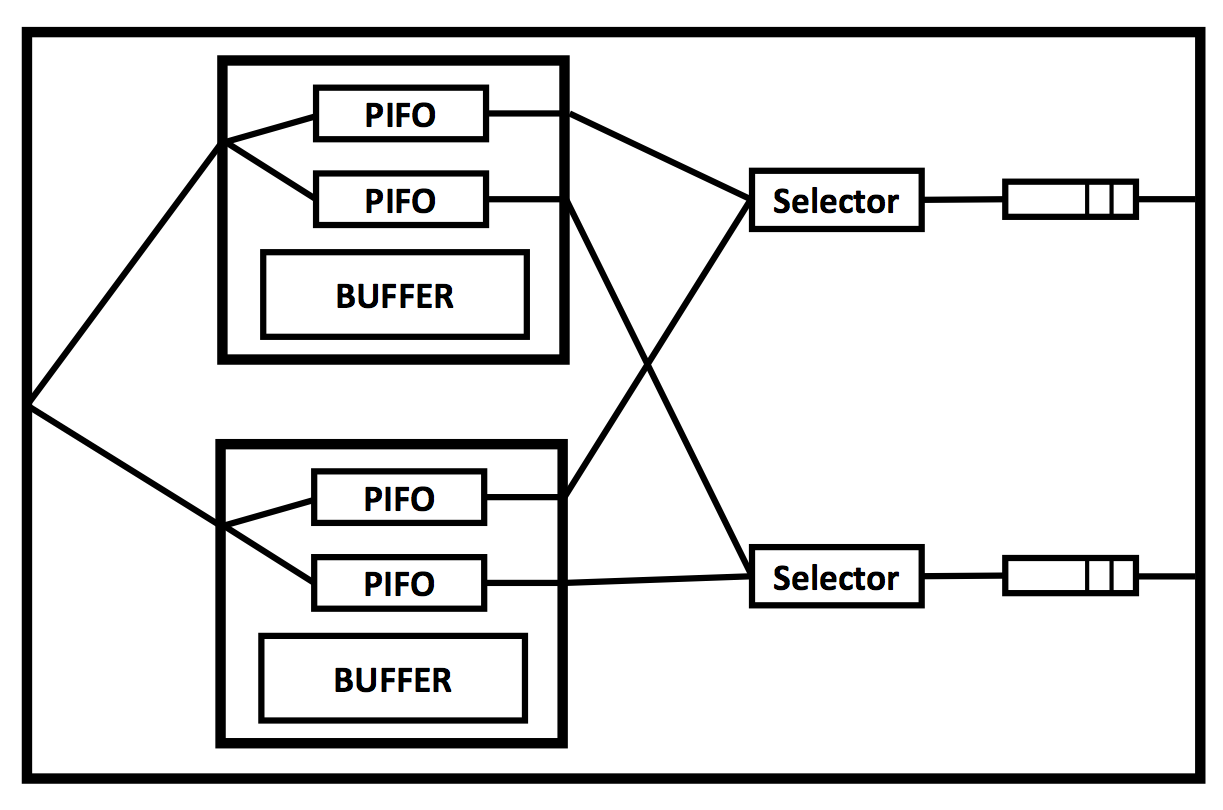
\includegraphics[width=1\linewidth]{figures/design/tm-top}
\caption{Top level traffic manager}
\label{fig:tm-top}
\end{figure}

\subsubsection{Packet Buffer}

The packet buffer consists of two BRAM modules, one to store 64B packet segments and another to store packet metadata. Unoccupied metadata slots and packet segments are accounted for using free lists. Packet segments are connected using a singly linked list.

Each input port is configured to have 130KB of packet segment storage (2048 segments); enough for about 100us of buffering, which is a typical RTT in datacenter networks~\cite{timely}. The packet buffer is designed to be the limiting resource at each input port. In other words, there will always be enough room in the PIFOs to store packet descriptors. Network operators often want to partition the available buffer space into some number of queues. These queues are used to isolate different classes of traffic, such that one does not consume the buffer space of another. In our design, the number of queues and their sizes are fully configurable. Queue sizes are enforced using simple counters which track the number of packet segments currently being consumed by each queue. Our design implements the tail drop policy; if a packet arrives destined for queue $N$ and the counter for queue $N$ has reached its maximum configured value then the packet is dropped.

While the design currently uses a static partitioning of buffer space into queues, in practice, this allocation would like be dynamic. This would simply require updating the control registers that are used to configure the queue allocations in our design. Furthermore, large FPGA memories or external RAM can be used to increase the size of the packet buffer.

